\documentclass{beamer}

\usepackage[ngerman]{babel}
\usepackage[utf8]{inputenc}

\mode<presentation>
{
  \usetheme[compress]{Torino}
}

\newcommand{\concept}[2]{
  \begin{block}{#1}
    #2
  \end{block}
}
\newcommand\startitemizeframe{\begin{itemize}}
\newcommand\stopitemizeframe{\end{itemize}}

\newenvironment{itemizeframe}[1]
  {\begin{frame}{#1}\startitemizeframe}
  {\stopitemizeframe\end{frame}}

\newcommand{\pattern}[2]{
  \begin{alertblock}{Problem}
    #1
  \end{alertblock}
  \pause
  \begin{exampleblock}{Lösung}
    #2
  \end{exampleblock}
}

\title{Hackerspace Design Patterns}

\author[Mic]{Mic \flq nomaster@chaosdorf.de\frq}

\institute[niemandsland]{Niemandsland e.V.}

\date[]{5. März 2012}

\begin{document}

  \begin{frame}
    \titlepage
  \end{frame}

  \begin{frame}{Übersicht}
    \tableofcontents
  \end{frame}

  \section{Einführung}

  \subsection{Begriffe}

  \begin{frame}{Ort}
    \concept{Hackerspace}{
      Ein \textsl{Hackerspace} ist ein physischer, kollektiv betriebener Raum,
      in dem Menschen sich treffen können und an ihren Projekten arbeiten.
    }
  \end{frame}

  \begin{frame}{Menschen}
    \concept{Hacker}{
      In einem übergreifenden Sinn umfasst \textsl{Hacker}
      experimentierfreudige Personen, die mit ihren Fachkenntnissen eine
      Technologie beliebiger Art außerhalb ihrer normalen Zweckbestimmung oder
      ihres gewöhnlichen Gebrauchs benutzen.
    }
  \end{frame}

  \begin{itemizeframe}{Aktivitäten}
    \item Do It Yourself
    \item Workshops
    \item Vorträge
    \item Teilen von Wissen
    \item Spaß haben
  \end{itemizeframe}

  \begin{itemizeframe}{Infrastruktur}
    \item Strom
    \item Computer-Netzwerk
    \item Internetzugang
    \item Werkzeuge
    \item Getränke
  \end{itemizeframe}

  \subsection{Bestehende Projekte}

  \begin{frame}{Noisebridge}
    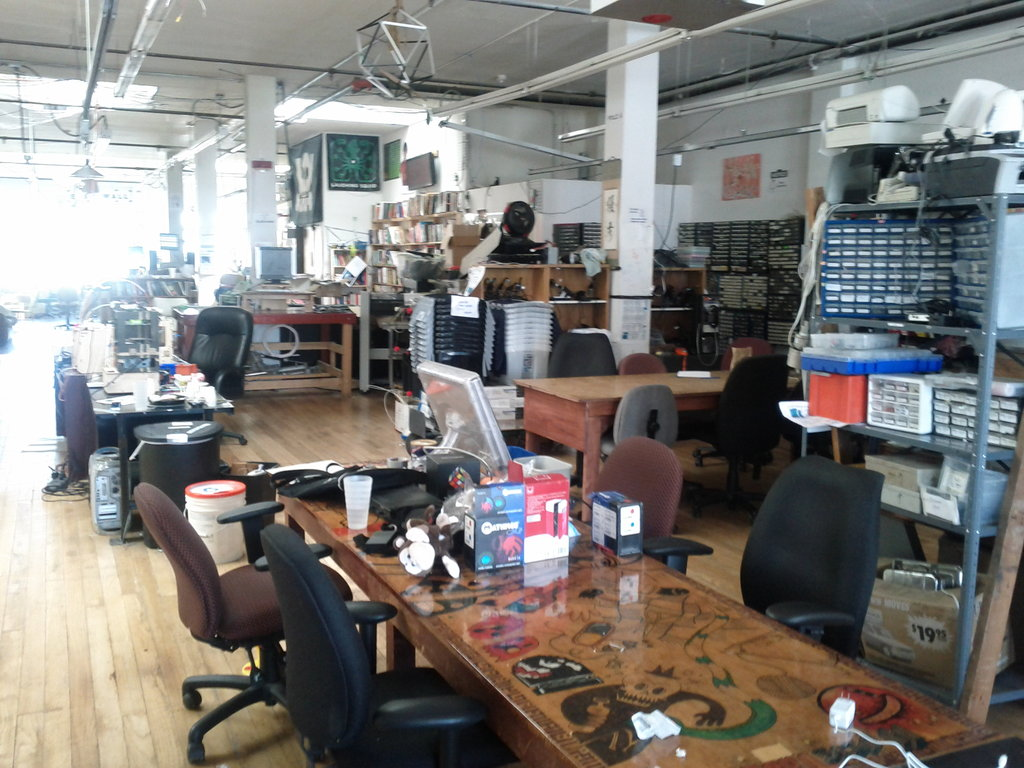
\includegraphics{noisebridge.jpg}
  \end{frame}

  \begin{frame}
    \begin{columns}[l]
      \column{.5\textwidth}
      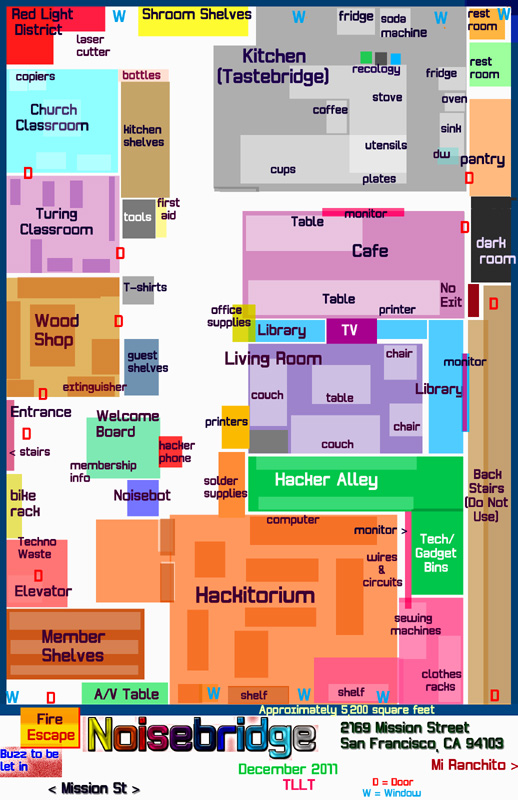
\includegraphics[width=0.9\textwidth]{noisebridge-map.jpg}
      \column{.5\textwidth}
      \begin{itemize}
        \item Gegründet 2007\\in San Francisco
        \item 483 $m^2$ Großraum
        \item 2 Seminarräume
        \item Hackcenter
        \item Laser-Labor
        \item Holzwerkstatt
        \item Schneiderrei
        \item Küche
        \item Café
        \item Wohnzimmer
      \end{itemize}
    \end{columns}
  \end{frame}

  \begin{frame}{Das Labor}
    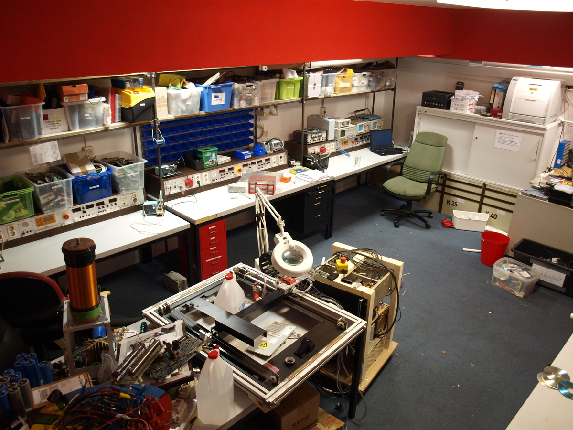
\includegraphics{daslabor.pdf}
  \end{frame}

  \begin{frame}
    \begin{columns}[l]
      \column{.5\textwidth}
      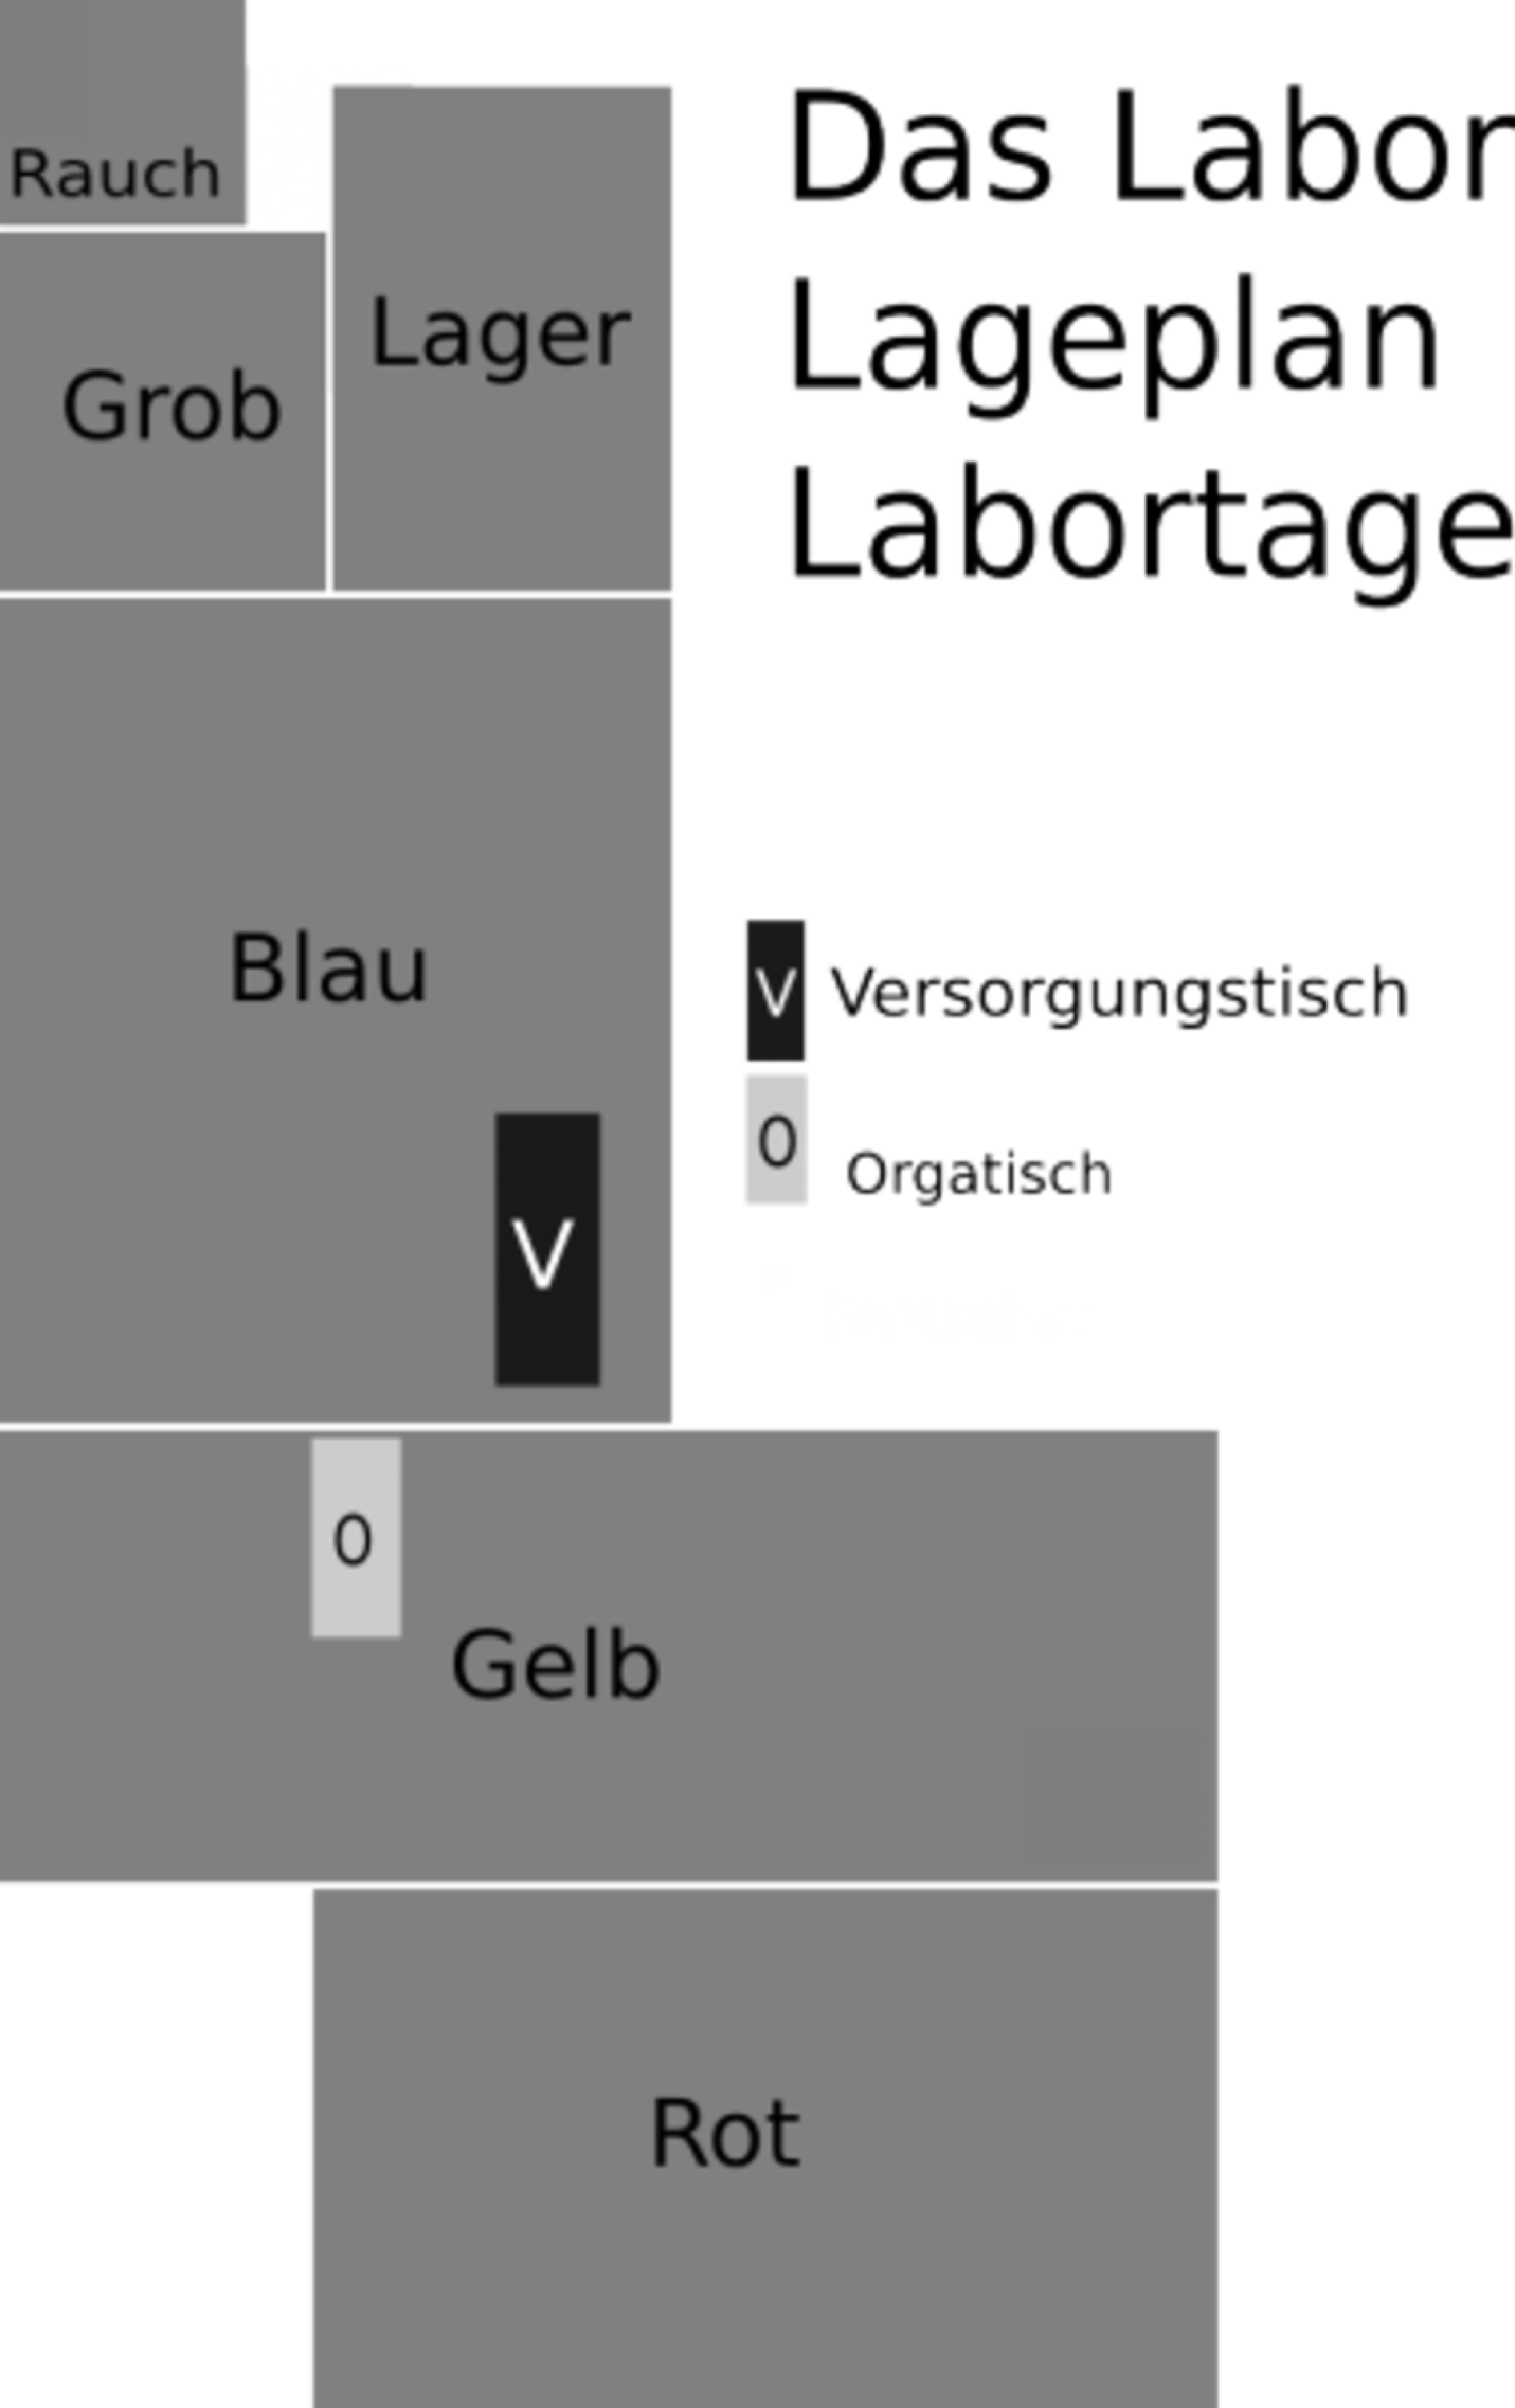
\includegraphics[width=0.9\textwidth]{daslabor-map.pdf}
      \column{.5\textwidth}
      \begin{itemize}
        \item Gegründet 2007\\in Bochum
        \item ca. 180 $m^2$
        \item Seminarraum (Blau)
        \item Elektronik-Werkstatt (Rot)
        \item Metallwerkstatt (Grob)
        \item Küche (Blau)
        \item Wohnzimmer (Gelb)
        \item Raucherzimmer (Rauch)
      \end{itemize}
    \end{columns}
  \end{frame}

  \subsection{Muster und Antimuster}

  \begin{frame}{Design Pattern}
    \concept{Entwurfsmuster}{Bewährte Lösungsschablonen für bestimmte, wiederkehrende Probleme}
  \end{frame}

  \begin{frame}{Anti-Pattern}
    \concept{Antimuster}{Häufig anzutreffende schlechte Lösungsansatze für bestimmte Probleme}
  \end{frame}

  \section{Hackerspaces Design Patterns}

  \subsection{Nachhaltigkeit}

  \begin{frame}{Infrastruktur}
    \pattern{
      Huhn oder Ei:\\
      Was sollte zuerst realisiert werden?\\
      Infrastruktur oder Projekte?
    }{
      Alles sollte von der Infrastruktur getragen werden. Räume, Strom, Server,
      Netzwerk und andere Einrichtungen haben Vorrang. Wenn du das erstmal hast,
      werden Menschen aufkreuzen und die verblüffensten Projekte an den Start
      bringen.
    }
  \end{frame}

  \begin{frame}{Grace Hopper}
    \pattern{
      Sollten wir den Space wirklich jetzt aufmachen?\\
      Haben wir an alles gedacht?
    }{
      \textbf{Ja klar!!!}
      \pause
      \begin{quote}
        Es ist immer einfacher hinterher um Vergebung zu bitten, als vorher um
        Erlaubnis.
      \end{quote}
      \pause
      Wichtig ist, den Start zu machen. Viele Probleme werden verschwinden, wenn
      du erst einmal angefangen hast.\\ \textbf{Im Zweifel: tu es!}
    }
  \end{frame}

  \begin{frame}{Kollektiv}
    \pattern{
      Wie sollte die Gruppe kommunizieren?
    }{
      Ihr seid Hacker. Ihr wisst, was zu tun ist. Hört auf, rumzuhängen und sezt
      eine Mailingliste auf. Und ein Wiki. Und einen IRC-Kanal. Alle drei werdet
      ihr brauchen. Denkt dabei an eine \textbf{Plattform für Diskussionen},
      Speicher für \textbf{Dokumentation} und \textbf{Echtzeit-Kommunikation}.
    }
  \end{frame}

  \begin{frame}{Kritische Masse}
    \pattern{
      Du willst als einziger in deiner Stadt einen Hackerspace eröffnen.
    }{
      Die Daumenregel lautet: \textbf{2 + 2}. Du brauchst einen Partner, um die
      Idee ans Laufen zu kriegen. Um die Arbeit zu schaffen, brauchst du noch
      zwei Leute mehr. Fange nicht an, wenn du nicht wenigstens 4 Leute dabei
      hast. Ab da ist es einfach, mehr Menschen zu rekrutieren. Um die zehn
      Leute sind ein guter Anfang.
    }
  \end{frame}

  \begin{frame}{Starke Persönlichkeiten}
    \pattern{
      Nichts wird fertig. Alle wollen den Hackerspace, aber ihr tut euch
      schwer, den Arsch hochzukriegen.
    }{
      Suche nach \textbf{starken Persönlichkeiten} als Mitglieder für deine
      anfängliche Gruppe. Du wirst Menschen brauchen, die \textbf{Erfahrungen
      mit dem Aufbau von Strukturen} haben. Schaue nach Menschen, die
      Autorität \textbf{besitzen} (und Respekt bekommen), nicht nach Menschen,
      die Autorität \textbf{ausnutzen} (und ausgelacht werden).
    }
  \end{frame}

  \subsection{Unabhängigkeit}

  \begin{frame}{Hausbesitzer und Nachbarschaft}
    \pattern{
      Du hast den perfekten Raum gefunden, aber der Hausbesitzer scheint
      merkwürdig zu sein. Außerdem sind die Nachbarn meckrig.
    }{
      Wähle weise. Ein großzügiger, aber uninteressierter Hausbesitzer und coole
      Nachbarn können grundlegene Gründe dafür sein, ob ein Hackerspace ans
      Laufen kommt, oder nicht. Nicht so coole Nachbarn könnten um 2 Uhr morgens
      die Bullen rufen. Abhängig von euren Projekten wird das zu einem
      ernsthaften Problem. Als Hacker lebt ihr nicht den Lebensstil der
      Bevölkerungsmehrheit – also schaut nach coolen Nachbarn die auch komisch
      sind und nicht zur Mehrheit gehören.
    }
  \end{frame}

  \begin{frame}{Anti-Mitbewohner}
    \pattern{
      Ihr braucht viel Platz für Treffen, Werkstatt, Lagerraum und
      Arbeitsflächen für Materialien und Projekte. Um die Miete zu senken oder
      aus sympathie denkt ihr, dass es großartig wäre, wenn ein Mensch in eurem
      Space lebt. Aber irgendwie klappt das nicht, weil du die Werkstatt nicht
      mehr nutzen kannst.
    }{
      Übernachtungsgäste im Hackerspace sind voll OK. Aber \textbf{lasst keinen
      dort wohnen}. Wenn sein muss, schmeißt die Person raus.
    }
  \end{frame}

  \begin{frame}{Séparée}
    \pattern{
      Ihr wollt chillen, diskutieren oder in Kleingruppen arbeiten. Aber der
      Hauptraum ist voll besetzt: es sind einfach zu viele Leute im Space. Oder
      ihr wollt eine Zigarette rauchen, ohne die anderen zu stören.
    }{
      Seht euch nach einem Hackerspace um, der kleine, separate Räume aufweist.
      Benutzt \textbf{Vorhänge} oder \textbf{Türen}, um den Hauptraum von den
      anderen Zimmern zu trennen. Diese Zimmer können auch zum Rauchen in einem
      Nichtraucher-Space verwendet werden.
    }
  \end{frame}

  \begin{frame}{Küche}
    \pattern{
      Als menschliches Wesen benötigst du Nahrung. Als Hacker benötigst du
      Koffein und Nahrung zu ungewöhnlichen Uhrzeiten.
    }{
      Richtet euch eine \textbf{Küche} ein. Nichts verbindet Menschen so gut,
      wie gemeinsames \textbf{Kochen}. Stellt Kühlschränke mit
      \textbf{Club-Mate} auf. Der Verkauf von Getränken hilft euch, die Miete
      reinzubekommen. Investiert in das allerwichtigste Stück Hardware
      überhaupt: eine \textbf{Spülmaschine}. Besorgt euch \textbf{Tiefkühler}
      für Pizza und kauft vernünftiges \textbf{Küchen-Equipment}. Zeigt Nerds,
      wie man \textbf{echtes Essen} kocht.
    }
  \end{frame}

  \begin{frame}{Behaglichkeit}
    \pattern{
      All work and no play makes Jack a dull boy. Da muss noch was anderes sein,
      als Arbeitsplätze und Elektronikkrempel.
    }{
      Holt euch \textbf{Sofas, bequeme Stühle, Tische, Aschenbecher,
      stimmungsvolle Beleuchtung, ein Soundsystem, Beamer und Videospiele}.
      Pflanzen haben für uns nicht funktioniert.
    }
  \end{frame}

  \begin{frame}{Dusche}
    \pattern{
      Nach langen hacking sessions werdet ihr anfangen, komisch zu riechen.
      Außerdem scheinen die Gäste in eurem Space Körperpflege zu
      vernachlässigen.
    }{
      Der Hackerspace von Welt hat ein \textbf{Badezimmer} mit \textbf{Dusche}.
      Nach einer langen Nacht werdet ihr besten Ideen kriegen, während ihr unter
      der Dusche steht. Gäste aus anderen Spaces können so über mehrere Tage
      bleiben. Am besten stellt ihr auch eine Waschmaschine auf, um die
      schmuddeligen Handtücher loszuwerden.
    }
  \end{frame}

  \begin{frame}{Mitgliedsbeiträge}
    \pattern{
      Ihr braucht Geld für die Miete und Ausrüstung. Größere Projekte brauchen
      Unterstützung.
    }{
      \textbf{Sammelt regelmäßig Beiträge ein}. Macht niemals Ausnahmen. Wählt
      einen angemessenen Betrag und gewährt Ermäßigung für Studenten. Behaltet
      immer mindestens drei Monate Miete auf dem Konto. Immer, ohne Ausnahme.
      Wählt einen totalitaristischen Schatzmeister.
    }
  \end{frame}

  \begin{frame}{Anti-Sponsoring}
    \pattern{
      Ihr glaubt, dass es eine gute Idee ist, bei einer wohlgesonnenen Firma
      unterzukommen. Oder in einer Universität, weil die meisten von euch
      ohnehin Studis sind.
    }{
      Macht euch \textbf{niemals von externen Sponsoren abhängig}. Spenden sind
      zu begrüßen, aber bedenkt, dass Firmen pleite gehen und keiner von euch
      ewig studieren wird. Treffen in Unis grenzen Berufsschüler aus, sowie
      Menschen, die die universitäre Kultur nicht mögen. Keine Firma, ungeachtet
      wie nett sie ist, wird euch ohne Ende beschenken, ohne irgendwann
      Gegenleistungen zu erwarten. Das ist Kapitalismus…
    }
  \end{frame}

  \subsection{Regelmäßigkeit}

  \begin{frame}{Plenum}
    \pattern{
      Ihr wollt interne Konflikte lösen, demokratische Entscheidungsfindung
      ausüben, laufende Probleme und Pläne für die Zukunft besprechen.
    }{
      Trefft euch \textbf{regelmäßig} mit möglichst allen Mitgliedern. Nehmt
      euch eine \textbf{Tagesordnung} vor und setzt euch \textbf{Ziele}. Lasst
      Leute veantwortung über ihre Aufgaben übernehmen. Verfasst ein
      \textbf{Protokoll} der Sitzung und setzt es auf eure Mailingliste und/oder
      in euer Wiki. Legt euch auf das einzige Intervall ein, das funktioniert:
      \textbf{ein Mal pro Woche}. Ungewöhnliche Regelungen wie „erster Vollmond
      nacht dem dritten Freitag” funktionieren nicht. So ist das auch mit
      zweiwöchigen Intervallen oder ähnlichem.
    }
  \end{frame}

  \begin{frame}{Dienstag}
    \pattern{
      Jeder Wochentag ist ungünstig. Ihr findet keinen Tag, an dem alle Zeit
      haben. Irgendwer hat immer einen anderen Termin.
    }{
      Trefft euch am \textbf{Dienstag}. Weil ja alle Tage gleich schelcht sind,
      nehmt einfach den Dienstag. Ende der Diskussion.
    }
  \end{frame}

  \begin{frame}{OpenChaos}
    \pattern{
      Ihr wollt neue Leute anziehen und eine Verbindung zur äußeren Welt herstellen.
    }{
      Veranstaltet monatlich einen öffentlichen Vortrag oder einen Workshop.
      Ladet dazu mit eurer Ortszeit ein (kein UTC, CEST, EST, etc.). Ladet
      interessierte Besucher zu euren Treffen ein und sagt den komischen Leuten
      nichts davon.
    }
  \end{frame}

  \begin{frame}{U23}
    \pattern{
      Ältere Mitglieder machen ihren Abschluss oder heiraten. Euer Space braucht junges Blut.
    }{
      Rekrutiert junge Leute durch \textbf{Wettbewerbe}, die ihr organisiert, in
      Form eines \textbf{Kurses über mehrere Wochen}. Überwältigt sie mit den
      Problemen des Hardware- und Software-Hackings und lasst sie diese in Teams
      lösen. Bereitet euch auf den Wettbewerb vor und \textbf{leitet sie an},
      aber gebt den Menschen Raum zum Experimentieren. Zieht euch nach dem
      Aufsetzen der Teams zurück und lasst die klügsten der jungen Leute den
      Laden schmeißen.
    }
  \end{frame}

  \begin{frame}{Sinuskurve}
    \pattern{
      Ihr habt alles richtig gemacht. Ein paar schöne Events und eine tolle
      Zeit in eurem flauschigen Hackerspace liegen zurück. Nach einiger Zeit
      jedoch geht der Enthusiasmus zurück und die Projekte stagnieren.
    }{
      Enthusiasmus in Hackerspaces entwickelt sich \textbf{sinusförmig} mit einer
      Schleifenlänge von \textbf{vier Jahren}. Haltet den Hackerspace am Laufen,
      auch wenn der Wohlfühlfaktor an Feiertagen fehlt. Die Chancen stehen gut,
      dass der Space in zwei Jahren wieder fantastisch läuft. \textbf{Gebt nicht
      auf!} Vielleicht klopft ja bereits morgen ein aufregendes neues Mitglied
      an eure Tür.
    }
  \end{frame}

  \subsection{Konfliktlösung}

  \begin{frame}{Konsens}
    \pattern{
      Ihr müsst eine Entscheidung treffen, die die ganze Gruppe betrifft und
      wollt sicherstellen, dass niemand übergangen wird.
    }{
      Diskutiert beim wöchentlichen \textbf{Plenum}. Stimmt nicht ab!
      Diskutiert, bis \textbf{alle einverstanden} sind. Für manche Probleme ist
      dies die beste Vorgehensweise.
    }
  \end{frame}

  \begin{frame}{Demokratie}
    \pattern{
      Ihr müsst eine Entscheidung treffen, die die ganze Gruppe betrifft.
      Aber die Diskussion scheint nicht zu einer Einigung zu führen.
    }{
      Diskutiert beim wöchentlichen \textbf{Plenum}. Stimmt ab!
      \textbf{Die stärkste Minderheit dominiert die schwächeren Minderheiten}.
      Für manche Probleme ist dies die beste Vorgehensweise.
    }
  \end{frame}

  \begin{frame}{Befehl}
    \pattern{
      Niemand spült das Geschirr. Der Hackerspace sieht hulle aus. Keinen
      Menschen scheint das zu kümmern.
    }{
      \textbf{Befehle Leuten} das Geschirr zu reinigen, den Müll rauszubringen,
      die Infrastruktur am Laufen zu halten. \textbf{Schrei rum, wenn nötig.
      Aber mache immer mit.} Für manche Probleme ist dies die beste
      Vorgehensweise.
    }
  \end{frame}

  \begin{frame}{sudo}
    \pattern{
      Ihr habt als eine Gemeinschaft gleichgesinnter losgelegt, jedoch ist da
      draus plötzlich eine Diktatur eines einzelnen Hackers geworden.
    }{
      Vergebt keine Ränge. Nutzt Diktatur temporär, also für Projekte und wenn
      ihr es wirklich braucht. Habt keinen einzelnen Root-Benutzer.
    }
  \end{frame}

  \begin{frame}{Verantwortung}
    \pattern{
      Du hast dich freiwillig gemeldet, um eine bestimmte, kritische Komponente
      eurer Infrastruktur zu verantworten (z.B. den Mailserver). Jedoch hast du
      auf einmal das Bedürfnis rumzuhängen.
    }{
      Bloß weil freiwillige Mitarbeit nicht bezahlt wird, heißt das nicht, dass
      sie weniger wichtig ist. Denke dran, dass du so direkt deine Freunde und
      den Hackerspace verletzt. \textbf{Sei stolz auf deine freiwillige
      Mitarbeit}. Es wird dich als Person stärken und dich glücklich machen.
      Wenn du einmal merkst, dass du deinen Job nicht weiter machen kannst, ist
      eine letzte Aufgabe, \textbf{ihn zu übergeben}.
    }
  \end{frame}

  \begin{frame}{Diskussionskultur}
    \pattern{
      Ihr seid mitten in eurem wöchentlichen Plenum. Alle schreien und nichts
      wird fertig.
    }{
      Viele Geeks haben nur geringe Diskussionsfähigkeit, wegen jahrelanger Flamewars
      im Netz. Sorgt dafür, dass Menschen mit \textbf{echter Sozialkompetenz die
      Diskussion leiten}. Menschen, die Erfahrung in real life Politik gesammelt
      haben (wie z.B. Studierendenparlamente) waren für unsere Gruppen am
      zuträglichsten. \textbf{Lernt von ihnen. Und lernt, andere nicht zu
      unterbrechen.}
    }
  \end{frame}

  \begin{frame}{Anti-Fahrradschuppen}
    \pattern{
      Du schlägst eine neue Einrichtung für euren Hackerspace vor, wie z.B.
      einen Fahrradschuppen. Nun diskutieren alle über die Farbe. Und kein
      Fahrradschuppen wird gebaut.
    }{
      Das ist ein altbekanntes Problem. Wenn du etwas vorschlägst, was jeder
      andere in deinem Hackerspace bauen könnte, \textbf{werden sich alle an der
      Diskussion beteiligen}. Und wenn es nur die Farbe des Fahrradschuppens
      ist, oder das Design für eure T-Shirts, die Linux-Distro auf dem Server,
      etc. Nerds tendieren dazu, triviale Probleme in epischer Breite zu
      diskutieren und dabei komplexe Aufgaben zu ignorieren. \textbf{Markiert
      sinnlose Diskussionen} wie diese und beendet sie einfach.
    }
  \end{frame}

  \begin{frame}{Privatgespräch}
    \pattern{
      Jemand löst ein Problem aus, das nicht in der Gruppe gelöst werden kann.
    }{
      Lasst jemand erfahrenen der Gruppe mit dem Störer \textbf{privat reden}.
      \textbf{Höre der Person gut zu}. Teilt ihr mit, wie die Gruppe das Problem
      empfindet, ohne sie vor dieser zu exponieren.
    }
  \end{frame}

  \subsection{Kreatives Chaos}

  \begin{frame}{Alte Hardware}
    \pattern{
      Du willst geile neue Hardware anschleppen, aber es ist keine Ecke mehr
      frei. Dein Hackerspace ist ein Museum voller Müll geworden.
    }{
      Werft die alten, gebrauchten Dinge auf \textbf{einen Haufen}. Lasst alle
      Leute sich daran bedienen. Nach einer Weile \textbf{schmeißt ihr die
      Sachen weg}. Aber seid bedacht und \textbf{kündigt diesen Schritt an}.
      Nicht nur einmal, sondern drei mal in einem eskalierenden System.
    }
  \end{frame}

  \begin{frame}{Schlüssel zum Raum}
    \pattern{
      Du willst, dass der Space jederzeit zugänglich ist. Es ist keine Option,
      jemanden mitten in der Nacht anzurufen, nur um den Laden dicht zu machen,
      weil du nach Hause willst.
    }{
      \textbf{Händigt Schlüssel aus.} Notiert euch, wer einen Schlüssel hat.
      Besorgt euch ein \textbf{sicheres Schloss}, so dass keiner einen Schlüssel
      ohne Erlaubnis kopieren kann. Nehmt Pfand für die Schlüssel, so dass die
      Schlüsselhalter auf sie aufpassen. Ihr könnt euch auch ein feines
      elektronisches Schließsystem bauen (mit allen coolen Features und
      schmerzhaften Problemen)…
    }
  \end{frame}

  \begin{frame}{Club-Mate}
    \pattern{
      Ihr müsst Spenden sammeln. Ihr wollt nachts lange aufbleiben. Und ihr
      wollt einen richtig guten Eindruck machen, ohne Drogenkonsum.
    }{
      Kauft euch mindestens eine Palette \textbf{Club-Mate} und verkauft sie in
      eurem Hackerspace. Bald werdet ihr die Wirkung wahrnehmen.
    }
  \end{frame}

  \section{Ausblick}

  \subsection{Dies ist kein Kochbuch}

  \subsection{Vernetzung}

\end{document}
